\section{Use of the Operators in a Surveillance Camera System}
In this section, we use the operators defined previously to coordinate the heterogeneous model of a surveillance camera system. To do so, we propose to use \bflow to specify how the operators are applied on the models that compose the surveillance camera system. In the following, we first present the \bflow specification used to build the model of coordination for the surveillance camera system, and then, we execute the coordinated system. 

\subsection{\bflow Specification of the Surveillance Camera System}
To coordinate the surveillance camera system, we use \bflow to specify how the operators \emph{SyncFSMEventsAndActions}, \emph{startActivityWhenEnter} and \emph{AtomicActivity} are applied between the models in Figure~\ref{fig:camerasystem}. To specify this, we define a \bflow specification named \emph{CameraSystem} (Listing~\ref{lst:bflowcamerasystem}: line 1) that begins by importing the \bcool specification to use (Listing~\ref{lst:bflowcamerasystem}: line 2), and then, it specifies the models to coordinate (Listing~\ref{lst:bflowcamerasystem}: line 3 to 6).

\begin{lstlisting}[language=bflow,
caption={\bflow specification for the Surveillance Camera System},
label={lst:bflowcamerasystem}, 
basicstyle=\scriptsize\ttfamily, backgroundcolor=\color{LGrey}, numbers=left, xleftmargin=2pt]
BCOoLFlow CameraSystem
ImportBCOoL  "TFSMAndActivityHierarchical.bcool" ;
Model BatteryControl "batterycontrol.ad"
Model CameraControl "cameracontrol.tfsm"
Model doJPEG "doJPEGAlgorithm.ad"
Model doJPEG2000 "doJPEG2000.ad"
Flow 
	applies SyncFSMEventsAndActions between (BatteryControl, CameraControl);
	applies startActivityWhenEnter between (CameraControl, doJPEG);
	applies startActivityWhenEnter between (CameraControl, doJPEG2000);
	applies AtomicActivity between (CameraControl, doJPEG);		
	applies AtomicActivity between (CameraControl, doJPEG2000);		
end Flow;
\end{lstlisting}

The specification contains a set \emph{flows} that define which operator is applied and on which models. In the following, we describe each flow by presenting what operator is used and between which models is applied.  

The first flow (Listing~\ref{lst:bflowcamerasystem}: line 8) defines that the operator SyncFSMEventsAndActions is applied between the activity BatteryControl and the TFSM CameraControl. This results results in the synchronization of the corresponding Action and FSMEvent by relying on theirs names. 

The second and third flows define that the operator startActivityWhenEnter is applied first between the TFSM CameraControl and the activity doJPEG (Listing~\ref{lst:bflowcamerasystem}: line 9), and then, between the TFSM and the activity doJPEG2000 (Listing~\ref{lst:bflowcamerasystem}: line 10). This results in a synchronization between the entering and leaving of the states BatteryLow and BatteryHigh, and the execution of the activities doJPEG and doJPEG2000. 

To coordinate the time between the TFSMs and the activities, the fourth and fifth flows define that the operator AtomicActivity must be applied between the TFSM CameraControl and each activity (Listing~\ref{lst:bflowcamerasystem}: line 11 and 12). This results in a synchronization between the local clock of the TFSM CameraControl and the execution of the activities. 

In this subsection, we have present the \bflow specification for the surveillance camera system. The specification specified the order of application of the operators and on which models these operators are applied. In other words, the \bflow specification defines how to build the coordination model for camera system by relying on the operators previously defined. We want to highlight that these \bcool operators can be used to coordinate any set of TFSM and Activity models. In particular, in this subsection, we use these operators to coordinate the models of the camera by specifying the corresponding \bflow specification. In the following section, we use this specification to execute the coordinated system.    

\subsection{Execution of the Surveillance Camera System}

In the modeling workbench, we use the \bflow specification to coordinate the surveillance camera system. The resulting model of coordination is composed of six \ccsl relations. Then, we use the modeling workbench to execute the coordinated system. Figure~\ref{fig:camerasystem} illustrates the partial timing output of the execution of the camera. As a result of the coordination, the \mse \emph{BatteryisHigh:occurs} and \emph{BatteryisHigh:executeIt} are strongly synchronized (in red in Figure~\ref{fig:camerasystem}). When the camera is in BatteryHigh state (in magenta in Figure~\ref{fig:camerasystem}), the activity doJPEG2000 is allowed to execute and the time in the TFSM does not elapse (in cyan in Figure~\ref{fig:camerasystem}). Only when the activity is finished, the time can elapse thus the \mse \emph{ms:ticks} is allowed to tick. 

		\begin{figure}[h]
			\center
			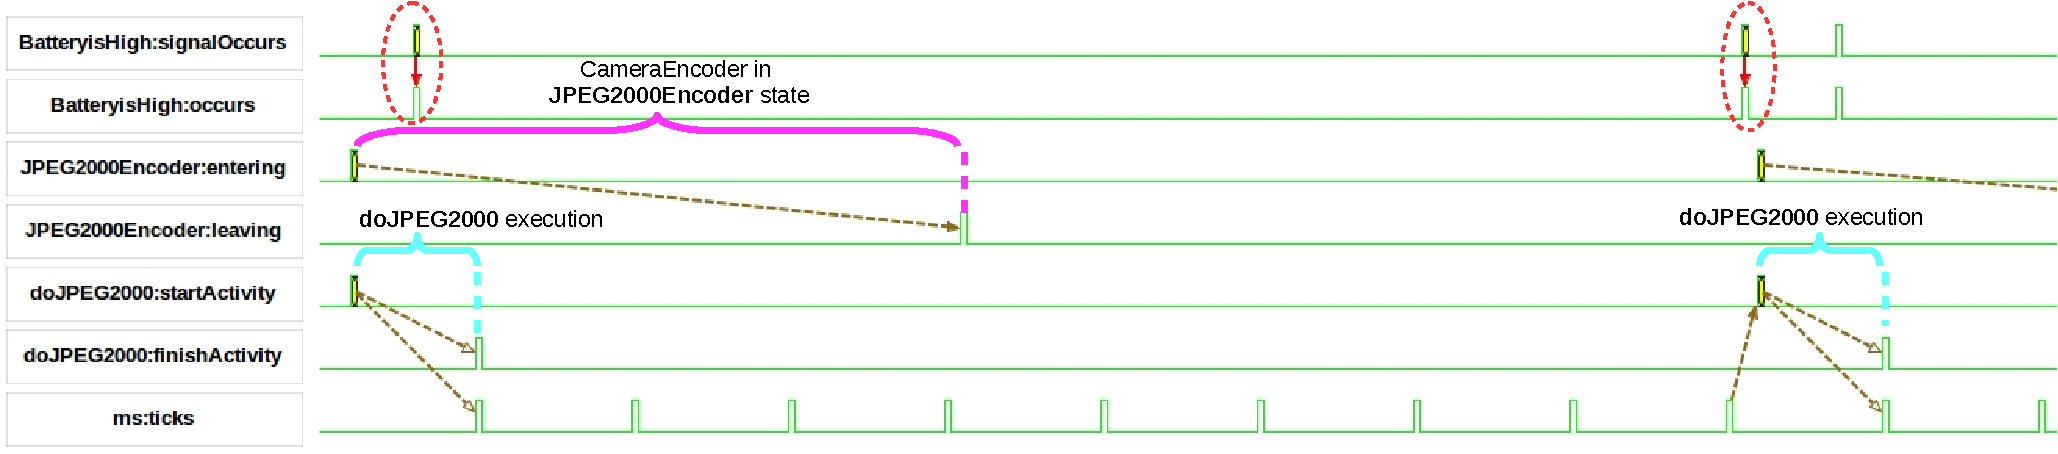
\includegraphics[width=1\columnwidth]{examples/figs/vcdcamera}
			\caption{Resulting timing output of the surveillance camera system}
			\label{fig:camerasystem}
		\end{figure}

%\todo{We want to highlighted that given the constrainst that we fixed and since all the states in the Camera are represented by activities, this makes the time not elapse at all. In the simulation, we only coordinated one of the activities, thus when the TFSM is in the other state the time is allowed to pass. The main drawback of this, is, since the activity as atomic, the time not elapse, this prevents the use of the timing transitions in the TFSM. In fact, there is non such a constrains, the time may elapse after the finishing of the activity and before the starting of it. However, this is hard to see that in the simulation, politic of the simulation?}

In this section, we have shown the use of \bflow to specify how the operators defined in the previous section are applied between the models of the camera. Then, we used this specification in the modeling workbench to execute the coordinated system. The reader can find the complete example in the companion website, which contains the models together with a detailed procedure to execute and verify the models. In addition, the site includes a video that shows the complete workflow by using the GEMOC studio. In the next section, we discuss about our approach by comparing it with coordination frameworks that propose a hard-coded hierarchical coordination.  
%the operator SyncProdut must be applied one time to coordinate the models … Then, the operators startActivityWhenEnter and AtomicActivity must be applied twice, one time for each activity. This specification is only for one camera which is composed by three models. However, this can be extended for N camera by modifying the bflow. 

	
	
	